\documentclass[../thesis.tex]{subfiles}
\newcommand{\subf}[2]{%
  {\small\begin{tabular}[t]{@{}m{.3\textwidth}@{}}
  #1\\ \centering #2
\end{tabular}}%
}\begin{document}
\chapter{Chemical Structures}\label{sec:structures}
\begin{longtable}{c c c}
\subf{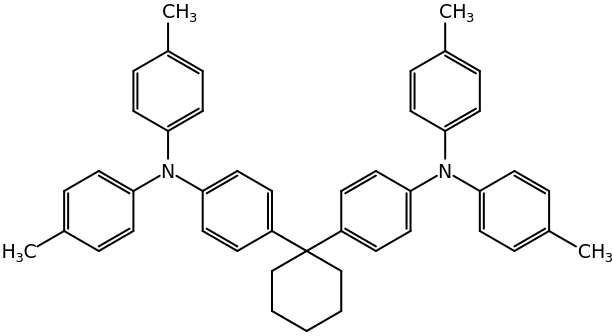
\includegraphics[width=.3\textwidth]{tapc}}
  {TAPC}
 & \subf{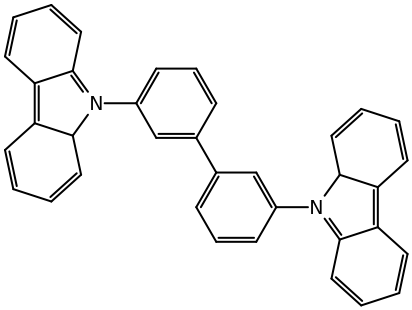
\includegraphics[width=.3\textwidth]{mcbp}}
  {mCBP}
 & \subf{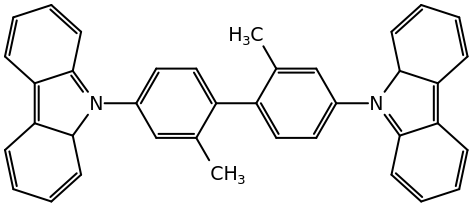
\includegraphics[width=.3\textwidth]{cdbp}}
  {CDBP}
\\\subf{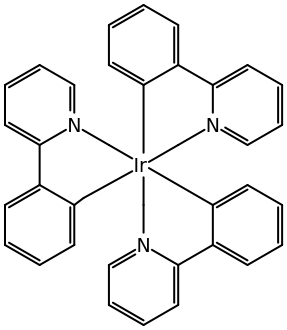
\includegraphics[width=.3\textwidth]{ir(ppy)3}}
  {Ir(ppy)3}
 & \subf{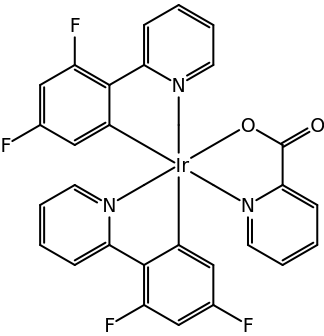
\includegraphics[width=.3\textwidth]{firpic}}
  {FIrpic}
 & \subf{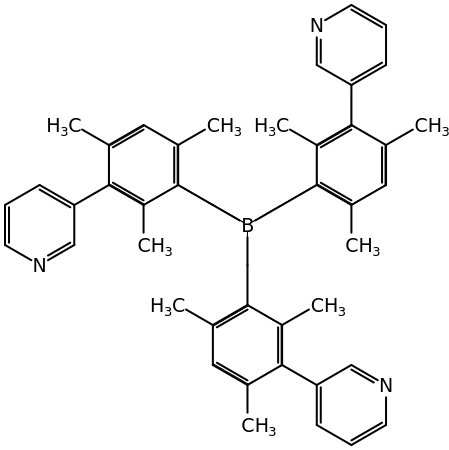
\includegraphics[width=.3\textwidth]{3tpymb}}
  {3TPYMB}
\\\subf{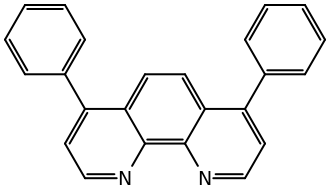
\includegraphics[width=.3\textwidth]{bphen}}
  {Bphen}
 & \subf{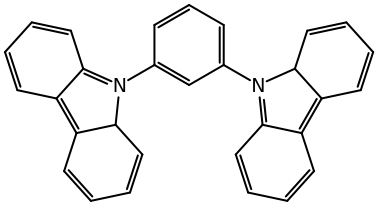
\includegraphics[width=.3\textwidth]{mcp}}
  {mCP}
 & \subf{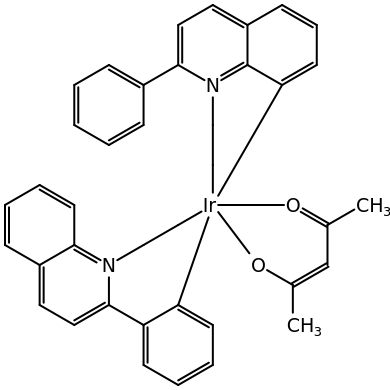
\includegraphics[width=.3\textwidth]{pqir}}
  {PQIr}
\\\subf{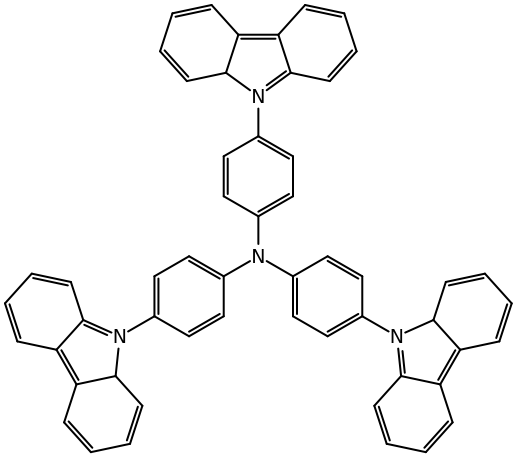
\includegraphics[width=.3\textwidth]{tcta}}
  {TCTA}
 & \subf{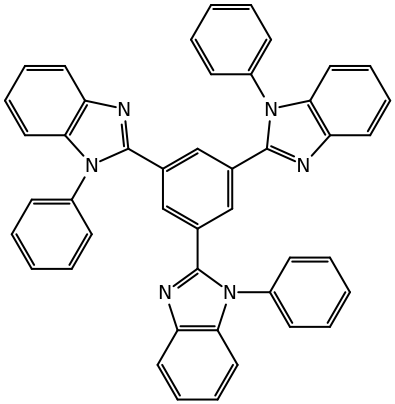
\includegraphics[width=.3\textwidth]{tpbi}}
  {TPBi}
 & \subf{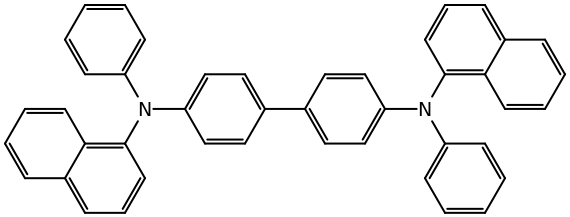
\includegraphics[width=.3\textwidth]{npd}}
  {NPD}
\\\subf{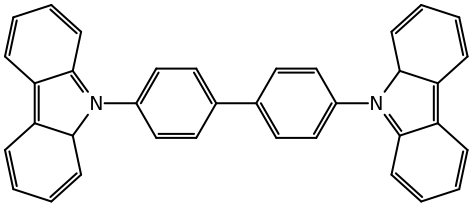
\includegraphics[width=.3\textwidth]{cbp}}
  {CBP}
 & \subf{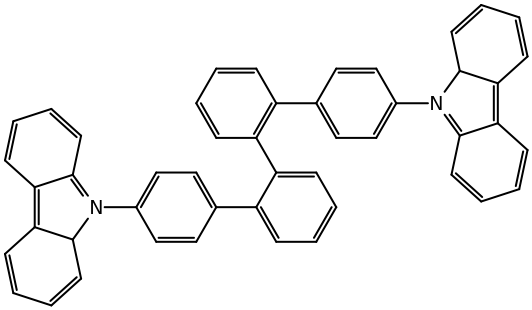
\includegraphics[width=.3\textwidth]{bcbp}}
  {BCBP}
 & \subf{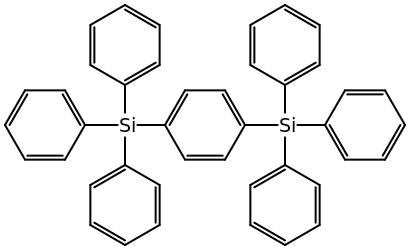
\includegraphics[width=.3\textwidth]{ugh2}}
  {UGH2}
\\\subf{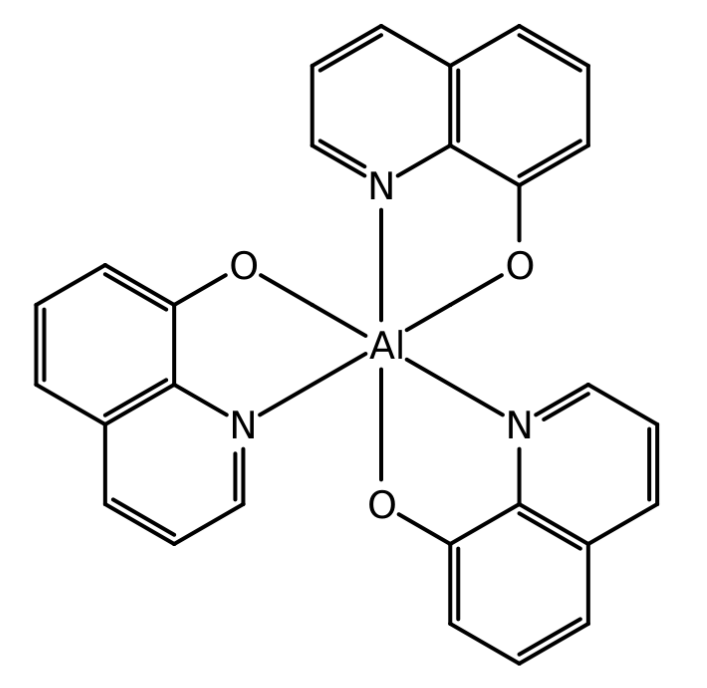
\includegraphics[width=.3\textwidth]{alq3}}
  {Alq3}
  \end{longtable}\end{document}
